\section{Design Considerations}
The design of the controller has to comply with the requirements from \autoref{requirements}. This is done to ensure that the design of the controller meets the desired performance. The requirements are listed as:\vspace{-0.6 cm}
\begin{itemize}
\item Steady state error: 0 \% \vspace{-0.2 cm}
\item Rise time: < 1 s \vspace{-0.2 cm}
\item Settling time: < 3 s \vspace{-0.2 cm}
\item Overshoot: < 10 \% \vspace{-0.2 cm}
\item Phase margin: $\geq 80 \degree$ \vspace{-0.2 cm}
\item Gain margin: $\geq 6$ dB 
\end{itemize}
The design of the controller will be based on these requirements and the model derived from the previous chapter. 
\subsection{Cascade Controller}
%The full system model is:
%\begin{equation}
%\frac{\Theta_p(s)}{V_a(s)}=\frac{0.8167148\cdot s}{s^3 +9.799\cdot s^2 -15.47\cdot s -151.59053} 
%\end{equation}
%From this it is clear, that the system is unstable due to the positive poles. The model is a third order and
%The model of the segway can be slit into two sub models, the motors and wheels model and the inverted pendulum model, as listed below. \\
%Motors and wheels model:
%\begin{equation}
%\frac{\omega_w(s)}{V_a(s)}=\frac{17.72}{s+9.799}
%\end{equation}
%The motors and wheels model is a first order system with a pole in -9.799. This means it is a type 0 system. This reveals some charateristics. One of them is, that there is a steady state error in its step response. \newpar
%Inverted pendulum model:
%\begin{equation}
%\frac{\Theta_p(s)}{\omega_w(s)}=\frac{0.04609\cdot s}{s^2 - 15.47}
%\end{equation}
%This is a second order model, with a positive pole. This system is therefore unstable, and this should be the first issue to adress when designing a controller. This model has a zero in zero. \newpar
When controlling a system where multiple sensors can be implemented, allowing feedback signals from different places in a process, cascade control is often a preferable way of controlling the system. This is because a cascade control improves robustness against disturbances and improves the dynamic performance of the system \citep{sou:cascade_controller}. It has therefore been decided to design a cascade controller. Loops within a cascade controller are coupled such that there is an outer and inner loop. If the inner loop's rise time is 3-5 times faster than the outer loop's, then the inner loop can be seen as having a transfer function of 1, when designing the outer loop \citep{sou:control_slide13}. This simplifies the design process of the outer loop considerably. %It shall be noted, that it is possible to design two control loops and connect them in series, but the advantages of coupling them in a cascade loop is predominant, see \autoref{fig:cascade}.\newpar
%The inner loop has to be 3-5 times faster than the outer loop, as it is assumed in the outer loop, that its input is equal to 1 due to obtained steady state in the inner loop. It shall be noted, that it is possible to design two control loops and connect them in series, but the advateges of coupling them in a cascade loop is predominant.\newpar
\begin{figure}[H]
\centering
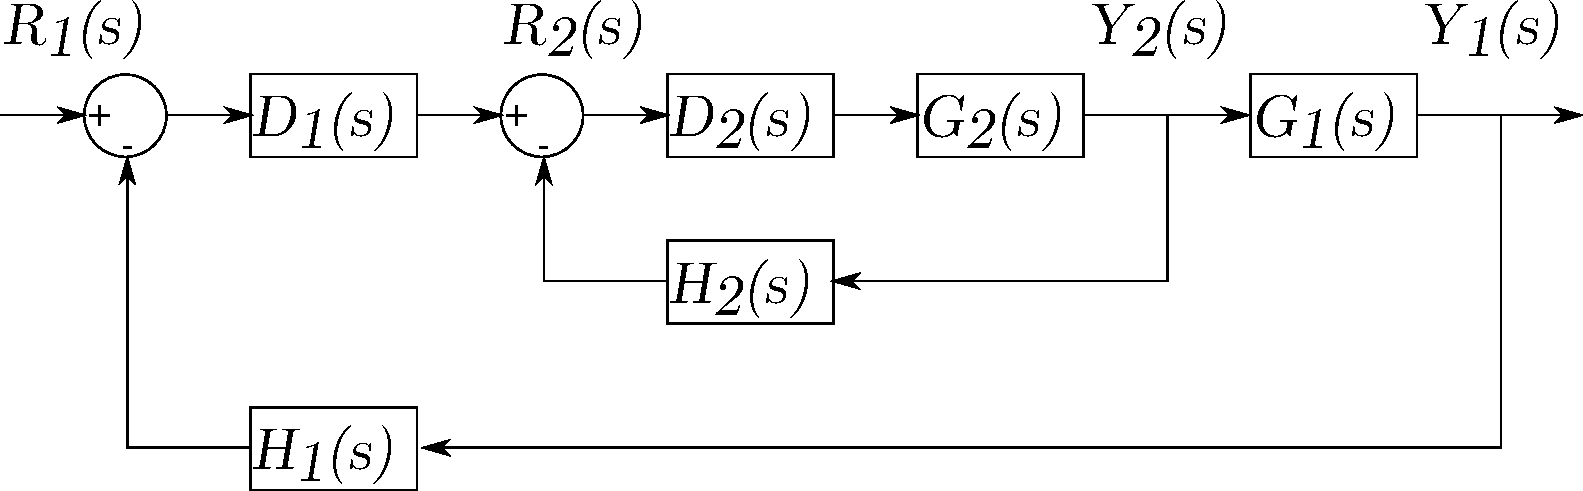
\includegraphics[scale=0.5]{figures/cascade.pdf}
\caption{Cascade control with two loops. \label{fig:cascade}} 
\end{figure}
\autoref{fig:cascade} displays a cascade control loop of two controllers. A cascade controller can hold more than two loops depending on how many sensor inputs are available in a system. %Step responses for a cascade control loop and a control loop with loops coupled in series are shown in \autoref{fig:cascadeseries}.
%\begin{figure}[H]
%\centering
%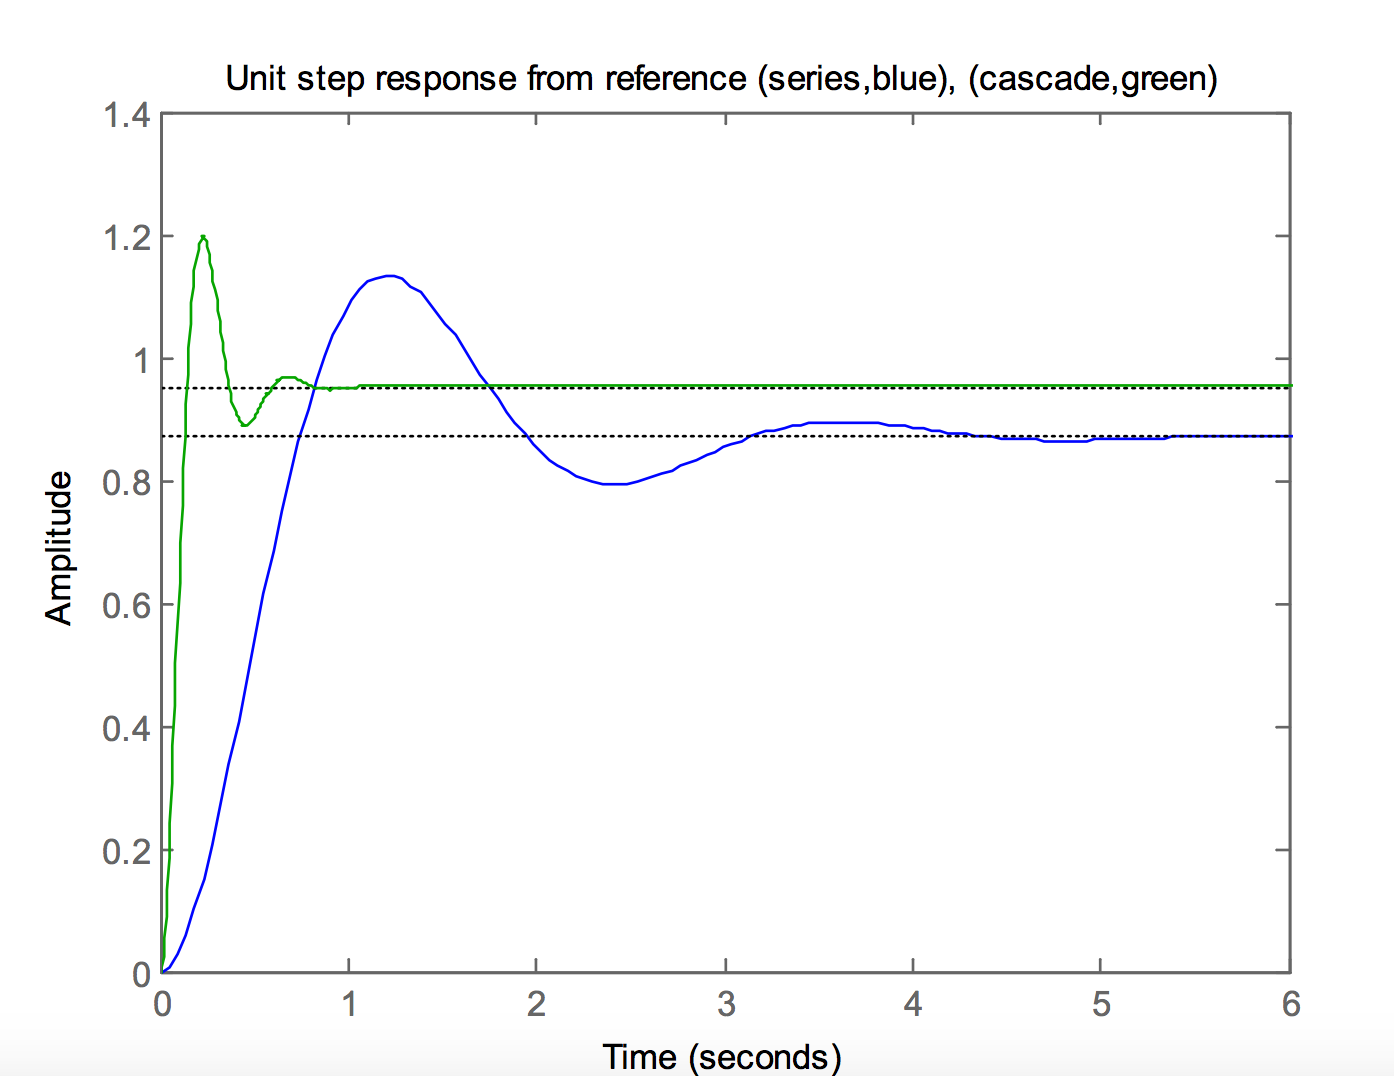
\includegraphics[scale=0.5]{figures/cascadeseries.PNG}
%\caption{Step response for sascade and series coupled loops. \label{fig:cascadeseries}} 
%\end{figure}
%\todo{Consider if it is right, that this figure is a comparison between a cascade and two loops in series. I don't think it is. Make new figure}
%From \autoref{fig:cascadeseries} it can be seen, that the cascade loop is significantly faster to settle and that it settles with a lower steady state error compared with the series loop. It also shows that the risetime is faster, however the overshoot is greater for the cascade controller. Concerning the requirements from \autoref{requirements}, it is prefferable to design a cascadecontroller due to the predominant advantages. It is therefore chosen to design a cascade controller.\newpar
When applying cascade control to the system of the segway, the inner loop consists of an inner loop controller, $D_2(s)$, the motors and wheels model, $G_2(s)$, along with the sensor block $H_2(s)$. The outer loop consists of an outer loop controller, $D_1(s)$, the inverted pendulum model, $G_1(s)$, along with $H_1(s)$, see \autoref{fig:cascade}.\\\\ 
A cascade controller is designed in the following section.